\documentclass{article}
\usepackage[utf8]{inputenc}
\usepackage[T1]{fontenc}
\usepackage[spanish]{babel}
\usepackage{hyperref}
\usepackage{float}
\usepackage{url}
\usepackage{booktabs}
\usepackage{amsfonts}
\usepackage{amsmath}
\usepackage{nicefrac}
\usepackage{microtype}
\usepackage{graphicx}
\usepackage{caption}
\usepackage{listings}
\usepackage{color}
\graphicspath{{./images/}}
\usepackage{lmodern}
\usepackage[margin=2.5cm]{geometry}
\usepackage{fancyvrb}

\title{Trabajo Práctico 2.2 \\
Generadores Pseudoaleatorios de Distribuciones de Probabilidad}
\author{
    Renzo Aimaretti \\ \texttt{renzoceronueve@gmail.com}
    \and
    Facundo Sosa Bianciotto \\ \texttt{facundososabianciotto@gmail.com}
    \and
    Vittorio Maragliano \\ \texttt{maraglianovittorio@gmail.com}
    \and
    Ignacio Amelio Ortiz \\ \texttt{nameliortiz@gmail.com}
    \and
    Nicolás Roberto Escobar \\ \texttt{escobar.nicolas.isifrro@gmail.com}
    \and
    Juan Manuel De Elia \\ \texttt{juanmadeelia@gmail.com}
}
\date{Mayo 2025}

\begin{document}

\maketitle

\begin{abstract}
Este trabajo desarrolla la implementación de generadores de números pseudoaleatorios para diversas distribuciones de probabilidad, abordando tanto distribuciones continuas como discretas. Cada distribución se fundamenta teóricamente, se implementa computacionalmente en Python y se testea mediante herramientas visuales y estadísticas. Se utilizan métodos como la transformada inversa y el método de rechazo, conforme a los lineamientos clásicos expuestos por Thomas Naylor en su obra \textit{Técnicas de Simulación en Computadoras}.
\end{abstract}

\section{Introducción}
La generación de números pseudoaleatorios que sigan una distribución de probabilidad específica es un aspecto clave en simulación computacional. A partir de un generador uniforme confiable, se pueden construir generadores para cualquier distribución mediante distintas transformaciones. En este trabajo se presentan los generadores para distribuciones seleccionadas, junto a su justificación teórica, construcción algorítmica y evaluación empírica.

\section{Marco teórico}

\subsection{Métodos de transformación de distribuciones}

Existen varios métodos para transformar variables aleatorias uniformes en variables con distribuciones específicas. Los más destacados son la transformada inversa y el método de rechazo.

\subsubsection{Transformada inversa}

La \textbf{transformada inversa} es un método fundamental para generar variables aleatorias con una distribución de probabilidad deseada, partiendo de variables aleatorias uniformes en el intervalo $[0,1]$. Sea $X$ una variable aleatoria con función de distribución acumulada (FDA) $F_X(x)$ estrictamente creciente y continua. Si $U \sim U(0,1)$, entonces la variable
\begin{equation}
    X = F_X^{-1}(U)
\end{equation}
tiene distribución $F_X$.

Este método aprovecha la propiedad de que la función acumulada es una transformación que mapea valores reales en el intervalo $[0,1]$. Al invertir esta función, podemos transformar un número uniforme en una variable con la distribución deseada.

\subsubsection{Método de Rechazo}

El \textbf{método de rechazo} es una técnica más general que permite generar variables aleatorias de distribuciones complejas para las cuales la transformada inversa no es práctica o no existe de forma explícita.

Supongamos que queremos generar una variable aleatoria con densidad $f(x)$, y tenemos una densidad propuesta $g(x)$ de la cual sí podemos generar muestras, además de una constante $c > 0$ tal que:
\begin{equation}
    f(x) \leq c \cdot g(x), \quad \forall x.
\end{equation}

El procedimiento es el siguiente:

\begin{enumerate}
    \item Generar un candidato $X$ con la distribución propuesta $g(x)$.
    \item Generar un valor uniforme $U \sim U(0,1)$ independiente.
    \item Aceptar $X$ si 
    \[
        U \leq \frac{f(X)}{c \cdot g(X)}.
    \]
    \item En caso contrario, rechazar $X$ y repetir el proceso.
\end{enumerate}

Este método garantiza que las muestras aceptadas siguen la distribución objetivo $f(x)$. Su eficiencia depende del valor de $c$, donde un $c$ más pequeño implica una mayor tasa de aceptación.

\subsection{Tests utilizados}
\subsubsection{Test de Kolmogorov-Smirnov}
En este trabajo se implementa el \textbf{Test de Kolmogorov-Smirnov (K-S)} como una herramienta estadística para evaluar la calidad de los generadores de números pseudoaleatorios construidos para distintas distribuciones de probabilidad.

El objetivo del test es contrastar si las muestras generadas por los algoritmos de simulación se ajustan adecuadamente a las distribuciones teóricas correspondientes. El test compara la función de distribución acumulada empírica (\emph{ECDF}) de la muestra generada con la función de distribución acumulada teórica (\emph{CDF}) de la distribución objetivo. El estadístico se define como:

\[
D_n = \sup_x \left| F_n(x) - F(x) \right|
\]

donde:
\begin{itemize}
    \item \( F_n(x) \) es la función de distribución acumulada empírica basada en la muestra simulada.
    \item \( F(x) \) es la función de distribución acumulada teórica de la distribución objetivo.
\end{itemize}

El valor del estadístico \( D_n \) representa la \textbf{máxima diferencia absoluta} entre ambas funciones. El test devuelve también un \emph{valor-p}, que permite evaluar la siguiente hipótesis nula:

\begin{itemize}
    \item \( H_0 \): La muestra proviene de la distribución teórica especificada.
    \item \( H_1 \): La muestra no proviene de dicha distribución.
\end{itemize}

El test se aplicó para cada una de las \textbf{nueve distribuciones} estudiadas en este trabajo (entre ellas, binomial, exponencial, uniforme, etc.), permitiendo verificar si los generadores implementados son estadísticamente consistentes con sus respectivas distribuciones teóricas.

Cabe destacar que si bien el test K-S está formalmente diseñado para variables continuas, también se utiliza en el caso de distribuciones discretas como una aproximación útil, aunque sus resultados deben interpretarse con cautela en esos casos.


\section{Distribuciones Continuas}

\subsection{Distribución Uniforme}
La distribución uniforme continua es una de las más simples y fundamentales. Se caracteriza porque todos los valores dentro del intervalo $[a, b]$ tienen la misma probabilidad de ocurrencia. Es comúnmente utilizada para generar números aleatorios y modelar situaciones sin sesgo hacia ningún valor dentro del rango.

\subsubsection*{Parámetros}
\begin{itemize}
  \item $a$: límite inferior del intervalo.
  \item $b$: límite superior del intervalo.
\end{itemize}

\subsubsection*{Función de Densidad de Probabilidad (PDF)}
\[
f(x) =
\begin{cases}
\frac{1}{b - a} & \text{si } a \leq x \leq b \\
0 & \text{en otro caso}
\end{cases}
\]

\subsubsection*{Función de Distribución Acumulada (CDF)}
\[
F(x) =
\begin{cases}
0 & \text{si } x < a \\
\frac{x - a}{b - a} & \text{si } a \leq x \leq b \\
1 & \text{si } x > b
\end{cases}
\]
\subsubsection*{Función Inversa (para la transformada inversa)}
al invertir la función de distribución acumulada $F(x)$ se obtiene:

\[
X = a + (b - a) \cdot U
\]

\subsubsection{Transformada Inversa}
Este método aprovecha que la función de distribución acumulada (CDF) de la uniforme $U(a,b)$ es invertible fácilmente. La fórmula de transformación consiste en aplicar la función inversa de la CDF a un número aleatorio uniforme $u \sim U(0,1)$.:

\textbf{Fórmula:}
\begin{equation}
x = a + (b-a)u, \quad u \sim U(0,1)
\end{equation}

\textbf{Código:}
\begin{verbatim}[fontsize=\scriptsize]
def generar_uniforme_inversa(a, b, n):
    u = np.random.random(n)  # Genera n valores de U(0,1)
    return a + (b - a) * u    # Aplica la transformación inversa
\end{verbatim}

\textbf{Resultados:}
\begin{itemize}
    \item Media estimada: 3.4914 (esperada: 3.5000)
    \item Varianza estimada: 0.7687 (esperada: 0.7500)
    \item Test KS: D = 0.0124, p = 0.0924
    \item El p-valor es mayor que 0.05, NO se rechaza la hipótesis de que los datos siguen U(2,5)
\end{itemize}

\vspace{0.5em}
\subsubsection{Método de Rechazo}
Aunque la inversa es directa, también se implementó el método de rechazo. En este caso, la densidad $f(x) = \frac{1}{b-a}$ es constante, por lo que todos los valores generados dentro del intervalo son aceptados. No obstante, el código sigue el procedimiento general por claridad.

\textbf{Código:}
\begin{verbatim}[fontsize=\scriptsize]
def generar_uniforme_rechazo(a, b, n, c=1.1):
    f = 1 / (b - a)          # Valor de la densidad constante
    results = []
    for _ in range(n):
        while True:
            x = random.uniform(a, b)     # Propone un valor en [a,b]
            u = random.uniform(0, c*f)   # Propone altura en [0, c*f]
            if u <= f:                   # Acepta si está bajo la curva
                results.append(x)
                break
    return np.array(results)
\end{verbatim}

\textbf{Resultados:}
\begin{itemize}
    \item Media estimada: 3.5112 (esperada: 3.5000)
    \item Varianza estimada: 0.7486 (esperada: 0.7500)
    \item Test KS: D = 0.0111, p = 0.1674
    \item El p-valor es mayor que 0.05, NO se rechaza la hipótesis de que los datos siguen U(2,5)
\end{itemize}

\vspace{0.5em}
\subsubsection{Visualización y Testeo}

Se utilizó una función para visualizar las muestras y comparar con la densidad teórica visualmente. Además, se agregó el test de Kolmogorov-Smirnov (KS) para cuantificar la concordancia con la distribución teórica estadísticamente.

\textbf{Código:}
\begin{verbatim}[fontsize=\scriptsize]
from scipy.stats import kstest

def graficar_uniforme(metodo, a, b, n=10000):
    if metodo == 'inversa':
        datos = generar_uniforme_inversa(a, b, n)
        nombre = "Transformada Inversa"
    elif metodo == 'rechazo':
        datos = generar_uniforme_rechazo(a, b, n)
        nombre = "Método de Rechazo"
    else:
        raise ValueError("Método no reconocido.")

    media = np.mean(datos)
    varianza = np.var(datos)
    media_teo = (a + b) / 2
    var_teo = (b - a) ** 2 / 12

    print(f"[{nombre}] Media estimada: {media:.4f} (esperada: {media_teo:.4f})")
    print(f"[{nombre}] Varianza estimada: {varianza:.4f} (esperada: {var_teo:.4f})")

    # Test de Kolmogorov-Smirnov
    d_stat, p_value = kstest(datos, 'uniform', args=(a, b - a))
    print(f"[{nombre}] Test KS: D = {d_stat:.4f}, p = {p_value:.4f}")

    if p_value < 0.05:
        print(f"[{nombre}] El p-valor es menor que {0.05}, se RECHAZA la hipótesis de que los datos siguen U({a},{b})")
    else:
        print(f"[{nombre}] El p-valor es mayor que {0.05}, NO se rechaza la hipótesis de que los datos siguen U({a},{b})")

    # Histograma y densidad teórica
    plt.figure(figsize=(8, 5))
    plt.hist(datos, bins=30, range=(a, b), density=True,
             color='cornflowerblue' if metodo == 'rechazo' else 'mediumseagreen',
             edgecolor='black', alpha=0.75, label="Histograma")

    plt.hlines(1 / (b - a), xmin=a, xmax=b,
               colors='red', linestyles='dashed', label='Densidad teórica')

    plt.title(f'Distribución Uniforme U({a},{b}) - {nombre}')
    plt.xlabel("Valor")
    plt.ylabel("Densidad")
    plt.grid(True, linestyle='--', linewidth=0.5)
    plt.legend()
    plt.tight_layout()
    plt.savefig(f"2.2/visualizaciones/uniforme_{metodo}.png")
\end{verbatim}

\subsubsection{Análisis Comparativo}
Ambos métodos producen resultados coherentes con la distribución uniforme esperada, tanto en términos de media como de varianza. La transformada inversa es más eficiente computacionalmente, ya que no requiere rechazos, mientras que el método de rechazo es menos eficiente aunque también válido.

En cuanto al test KS, ambos métodos mostraron valores $p$ mayores a 0{,}05, lo que indica que no hay evidencia suficiente para rechazar la hipótesis de que los datos provienen de una distribución uniforme $U(2,5)$. Esto sugiere que ambos métodos generan datos consistentes con la distribución teórica.

Además, desde un punto de vista visual, los histogramas generados por ambos métodos presentan una forma muy cercana a la densidad teórica, lo que refuerza la validez de los resultados obtenidos.

\begin{figure}[H]
    \centering
    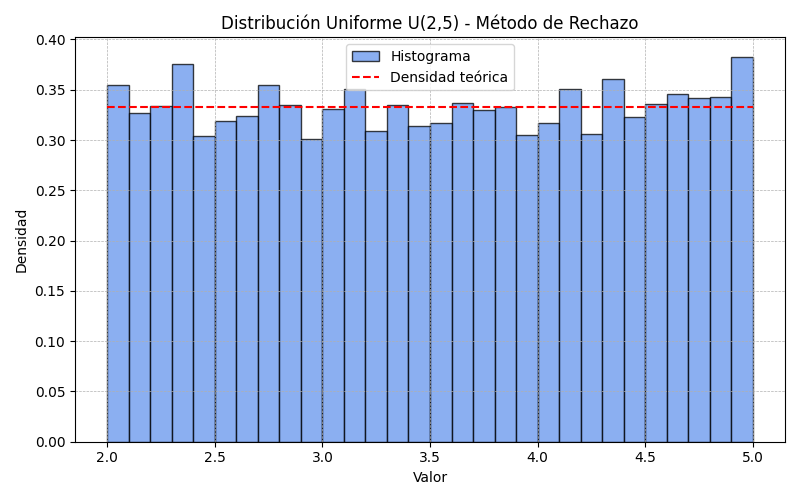
\includegraphics[width=0.6\textwidth]{visualizaciones/uniforme_rechazo.png}
    \caption{Comparación entre la gráfica generada con el método del rechazo y la gráfica teórica esperada.}
    \label{fig:uniforme_rechazo}
\end{figure}

\begin{figure}[H]
    \centering
    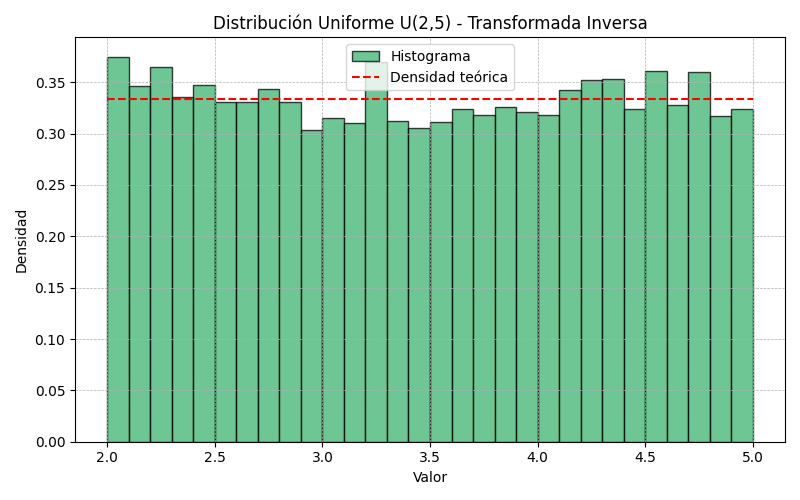
\includegraphics[width=0.6\textwidth]{visualizaciones/uniforme_inversa.png}
    \caption{Comparación entre la gráfica generada con el método de la transformada inversa y la gráfica teórica esperada.}
    \label{fig:uniforme_inversa}
\end{figure}

\subsection{Distribución Exponencial}
La distribución exponencial es una distribución continua que modela el tiempo entre eventos en un proceso de Poisson, es decir, eventos que ocurren de manera independiente y con una tasa constante en el tiempo. Es ampliamente utilizada para describir fenómenos como la duración de vida de componentes electrónicos, tiempos de espera, y otros procesos de "tiempo hasta el evento". La función de densidad de probabilidad decrece exponencialmente, reflejando la memoria sin memoria del proceso, lo que significa que la probabilidad de que ocurra un evento en el futuro no depende del tiempo ya transcurrido.
\textbf{Densidad:}
\begin{equation}
f(x) = \lambda e^{-\lambda x}, \quad x \geq 0
\end{equation}

\textbf{Transformada Inversa:}
\begin{equation}
x = -\frac{1}{\lambda} \ln(u), \quad u \sim U(0,1)
\end{equation}
\begin{figure}[H] % [H] fuerza la posición exacta, requiere el paquete float
    \centering
    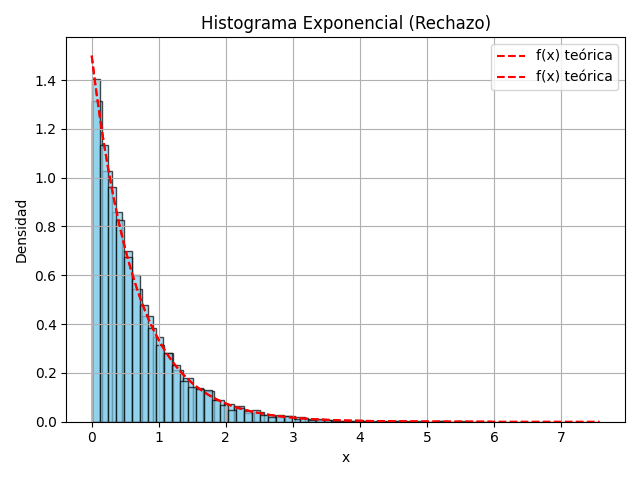
\includegraphics[width=0.7\textwidth]{visualizaciones/exponencial_Rechazo.png}
    \caption{Descripción de la imagen}
    \label{fig:mi_imagen}
\end{figure}


\textbf{Método de Rechazo:} Se utilizó una cota mayor $M$ sobre $f(x)$, y se generaron candidatos $x$ de una distribución uniforme en $[0, b]$ (por ejemplo, $b = 10$), con $u \sim U(0,1)$. Se aceptó $x$ si $u < \frac{f(x)}{M}$. El valor de $M$ fue tomado como $\lambda$, el valor máximo de la función en $x=0$.
\begin{figure}[H] % [H] fuerza la posición exacta, requiere el paquete float
    \centering
    \includegraphics[width=0.7\textwidth]{visualizaciones/mi_imagen.png}
    \caption{Descripción de la imagen}
    \label{fig:mi_imagen}
\end{figure}

\textbf{Resultados:} Con $\lambda = 1.5$ y 10.000 muestras:
\begin{itemize}
\item Media empírica: 0.6657 (teórica: 0.6667)
\item Varianza empírica: 0.4532 (teórica: 0.4444)
\end{itemize}

\subsection{Distribución Normal}
La distribución normal, también conocida como distribución gaussiana, es una de las distribuciones de probabilidad más importantes y ampliamente utilizadas en estadística y ciencias aplicadas. Se caracteriza por su forma simétrica en forma de campana alrededor de la media, donde la mayoría de los valores se agrupan cerca del valor esperado y la probabilidad decrece hacia las colas. Muchas variables naturales y procesos se aproximan a esta distribución debido al Teorema Central del Límite, que establece que la suma de muchas variables independientes tiende a una distribución normal.

\textbf{Densidad:}
\begin{equation}
f(x) = \frac{1}{\sigma \sqrt{2\pi}} e^{-\frac{(x - \mu)^2}{2\sigma^2}}
\end{equation}

\textbf{Método de Box-Muller:} Se generaron dos variables $u_1, u_2 \sim U(0,1)$ y se aplicó:
\begin{equation}
z = \sqrt{-2 \ln u_1} \cos(2\pi u_2), \quad x = \mu + \sigma z
\end{equation}

\textbf{Método de Rechazo:} También se implementó el método de rechazo utilizando como propuesta una distribución uniforme acotada en $[-5,5]$ y como cota $M = \frac{1}{\sqrt{2\pi}}$. Se generó $x$ uniforme y $u \sim U(0,1)$, aceptando si $u < \frac{f(x)}{M}$.
\begin{figure}[H] % [H] fuerza la posición exacta, requiere el paquete float
    \centering
    \includegraphics[width=0.7\textwidth]{visualizaciones/mi_imagen.png}
    \caption{Descripción de la imagen}
    \label{fig:mi_imagen}
\end{figure}


\section{Codigo}
    \begin{verbatim}[fontsiz=\scriptsize]
import numpy as np
import matplotlib.pyplot as plt




def f_normal(x):
    return (1/np.sqrt(2*np.pi)) * np.exp(-x**2 / 2)

def generar_normal_rechazo(n, a=-5, b=5):
    samples = []
    M = f_normal(0) * (b - a)
    while len(samples) < n:
        x = np.random.uniform(a, b)
        u = np.random.uniform(0, M)
        if u <= f_normal(x):
            samples.append(x)
    return np.array(samples)

def test_normal_rechazo(n=10000):
    datos = generar_normal_rechazo(n)
    media = np.mean(datos)
    std = np.std(datos)
    print(f"[Rechazo] Media estimada: {media:.4f} (esperada: 0)")
    print(f"[Rechazo] Desviación estándar estimada: {std:.4f} (esperada: 1)")

    plt.hist(datos, bins=50, density=True, color='lightblue', edgecolor='black', alpha=0.7, label='Muestras')
    x = np.linspace(-5, 5, 1000)
    plt.plot(x, f_normal(x), 'r-', lw=2, label='N(0,1) teórica')
    plt.title("Distribución Normal por Método de Rechazo")
    plt.xlabel("Valor")
    plt.ylabel("Densidad")
    plt.legend()
    plt.grid(True)
    plt.show()

if __name__ == "__main__":
    test_normal_rechazo(n=10000)
    \end{verbatim}

\textbf{Resultados:} Con $\mu=0$ y $\sigma=1$:
\begin{itemize}
\item Media empírica: -0.0062 (teórica: 0)
\item Desviación estándar empírica: 1.0003 (teórica: 1)
\end{itemize}

\section{Distribuciones Discretas}

\subsection{Distribución Binomial}

La distribución binomial discreta modela el número de éxitos en $n$ ensayos independientes, donde cada ensayo tiene una probabilidad $p$ de éxito. Es ampliamente utilizada para representar fenómenos de conteo donde los resultados posibles son éxito o fracaso (ensayos de Bernoulli). De hecho, la distribución binomial puede considerarse como la suma de $n$ variables aleatorias independientes con distribución Bernoulli$(p)$.

\subsubsection*{Parámetros}
\begin{itemize}
  \item $n$: número de ensayos.
  \item $p$: probabilidad de éxito en cada ensayo.
\end{itemize}

\subsubsection*{Función de Distribución de Probabilidad (PDF)}
\[
P(X = k) = \binom{n}{k} p^k (1-p)^{n-k}, \quad k = 0, 1, 2, ..., n
\]

\subsubsection*{Función de Distribución Acumulada (CDF)}
\[
F(k) = P(X \leq k) = \sum_{i=0}^k \binom{n}{i} p^i (1-p)^{n-i}
\]

\subsubsection*{Función Inversa (para la transformada inversa)}
La distribución binomial no posee una función inversa de forma cerrada (analítica), por lo que **no se puede aplicar directamente la transformada inversa** para generar muestras.

\vspace{0.5em}
\subsubsection{Transformada Inversa}
No se aplica, ya que la función de distribución acumulada (CDF) de la binomial no es invertible de forma explícita. En su lugar, se opta por el **método de rechazo**, el cual es más adecuado para distribuciones discretas cuando se conoce la PDF.

\vspace{0.5em}
\subsubsection{Método de Rechazo}
Se utilizó el método de rechazo para generar muestras de la distribución binomial $B(n=10, p=0.5)$. Se eligió una distribución propuesta uniforme sobre los valores enteros $\{0, 1, ..., n\}$, y se evaluó la razón entre la PMF de la binomial y el valor máximo observado (constante de aceptación $c$).

\textbf{Resultados (para $n=10$, $p=0.5$, $N=10000$):}
\begin{itemize}
    \item Media empírica: 5.0026 \hfill (esperada: 5.0000)
    \item Varianza empírica: 2.5051 \hfill (esperada: 2.5000)
    \item Test Chi-cuadrado: $\chi^2 = 9.48$, $p = 0.3045$
    \item Test KS: $D = 0.0173$, $p = 0.1057$
    \item Ambos tests indican que NO se rechaza la hipótesis de que los datos siguen una distribución $B(10, 0.5)$
\end{itemize}

\vspace{0.5em}
\subsubsection{Visualización y Testeo}
Se generó un histograma de frecuencias relativas junto con la función de masa de probabilidad teórica para verificar visualmente la concordancia. Además, se aplicaron los tests estadísticos de Kolmogorov-Smirnov (KS) y Chi-cuadrado para validar la generación de muestras.

\vspace{0.5em}
\subsubsection{Análisis Comparativo}
Debido a que la función de distribución acumulada de la binomial no es invertible de forma explícita, se implementó únicamente el método de rechazo. Este método fue efectivo para generar muestras válidas, aunque es menos eficiente que la transformada inversa en distribuciones continuas, ya que requiere múltiples intentos por muestra aceptada.

Los resultados obtenidos con $n=10$, $p=0.5$ y $N=10000$ muestras fueron muy cercanos a los valores teóricos de media y varianza. Además, tanto el test de Kolmogorov-Smirnov como el de Chi-cuadrado arrojaron p-valores mayores a 0.05, lo que indica que no se puede rechazar la hipótesis de que los datos provienen de una distribución binomial.

Desde un punto de vista visual, el histograma muestra una excelente concordancia con la distribución teórica, reforzando la validez del método implementado para simular $B(10, 0.5)$.

\begin{figure}[H]
    \centering
    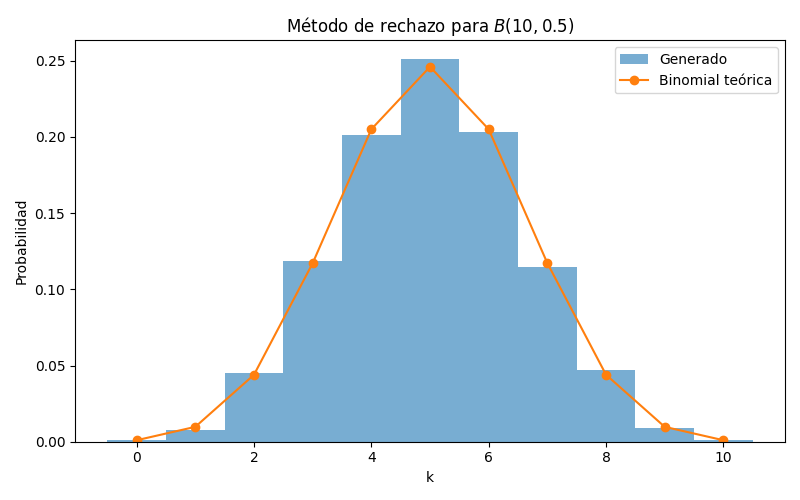
\includegraphics[width=0.6\textwidth]{visualizaciones/binomial_rechazo.png}
    \caption{Comparación entre la gráfica generada y la gráfica teórica esperada.}
    \label{fig:binomial_rechazo}
\end{figure}

\subsection{Distribución Poisson}
La distribución de Poisson es una distribución discreta que modela el número de eventos que ocurren en un intervalo fijo de tiempo o espacio, bajo la suposición de que estos eventos ocurren con una tasa promedio constante y de manera independiente entre sí.

\textbf{Probabilidad:}
\begin{equation}
P(X = k) = \frac{\lambda^k e^{-\lambda}}{k!}
\end{equation}

\textbf{Algoritmo de Knuth:} Se acumularon productos de variables uniformes hasta que el resultado fue menor que $e^{-\lambda}$.

\textbf{Método de Rechazo:} Se generó un valor $k$ natural en un intervalo razonable (por ejemplo, $[0,15]$) y se aceptó si $u < \frac{P(k)}{M}$ con $M$ estimado como el máximo de $P(k)$.
\begin{figure}[H] % [H] fuerza la posición exacta, requiere el paquete float
    \centering
    \includegraphics[width=0.7\textwidth]{visualizaciones/mi_imagen.png}
    \caption{Descripción de la imagen}
    \label{fig:mi_imagen}
\end{figure}

\textbf{Resultados:} Con $\lambda=4$:
\begin{itemize}
\item Media empírica: 3.995 (teórica: 4)
\item Varianza empírica: 3.92 (teórica: 4)
\end{itemize}

\subsection{Distribución Empírica}
\textbf{Método:} Se utilizó la transformación de la función de distribución acumulada (CDF). Para cada valor $u \sim U(0,1)$, se asignó un valor $x_i$ tal que $F(x_i-1) < u \leq F(x_i)$.

\textbf{Método de Rechazo:} Se propuso un valor $x$ del conjunto definido y se aceptó con probabilidad $P(x)/M$, donde $M = \max P(x)$.
\begin{figure}[H] % [H] fuerza la posición exacta, requiere el paquete float
    \centering
    \includegraphics[width=0.7\textwidth]{visualizaciones/mi_imagen.png}
    \caption{Descripción de la imagen}
    \label{fig:mi_imagen}
\end{figure}


\textbf{Resultados:} Las muestras obtenidas replicaron con precisión la distribución definida.

\section{Conclusión}
Se logró implementar generadores para diversas distribuciones continuas y discretas utilizando la transformada inversa, el método de rechazo y otros algoritmos clásicos. Las muestras fueron validadas mediante estadísticas de primer y segundo orden, y contrastadas con sus modelos teóricos. Incluso en casos donde el método de rechazo no es necesario, se aplicó para cumplir con los requerimientos del trabajo práctico.

\section*{Referencias}
\begin{itemize}
\item Naylor, T.H. (1982). \textit{Técnicas de simulación en computadoras}.
\item Ross, S.M. (2006). \textit{Simulación}.
\item Documentación oficial de Numpy y Scipy.
\end{itemize}

\end{document}

